%%%%%%%%%%%%%%%%%%%%%%%%%%%%%%%%%%%%%%%%%
% Stylish Article
% LaTeX Template
% Version 2.1 (1/10/15)
%
% This template has been downloaded from:
% http://www.LaTeXTemplates.com
%
% Original author:
% Mathias Legrand (legrand.mathias@gmail.com) 
% With extensive modifications by:
% Vel (vel@latextemplates.com)
%
% License:
% CC BY-NC-SA 3.0 (http://creativecommons.org/licenses/by-nc-sa/3.0/)
%
%%%%%%%%%%%%%%%%%%%%%%%%%%%%%%%%%%%%%%%%%

%----------------------------------------------------------------------------------------
%	PACKAGES AND OTHER DOCUMENT CONFIGURATIONS
%----------------------------------------------------------------------------------------

\documentclass[fleqn,10pt]{SelfArx} % Document font size and equations flushed left

\usepackage[english]{babel} % Specify a different language here - english by default
\usepackage{multirow}
\usepackage{fullpage}
\usepackage{graphicx}
\usepackage{amsthm}
\usepackage{amssymb}
\usepackage{url}
\usepackage{amsfonts}
\usepackage{algpseudocode}
\usepackage{mathtools}
\usepackage{lipsum} % Required to insert dummy text. To be removed otherwise

%----------------------------------------------------------------------------------------
%	COLUMNS
%----------------------------------------------------------------------------------------

\setlength{\columnsep}{0.55cm} % Distance between the two columns of text
\setlength{\fboxrule}{0.75pt} % Width of the border around the abstract

%----------------------------------------------------------------------------------------
%	COLORS
%----------------------------------------------------------------------------------------

\definecolor{color1}{RGB}{0,0,90} % Color of the article title and sections
\definecolor{color2}{RGB}{0,20,20} % Color of the boxes behind the abstract and headings

%----------------------------------------------------------------------------------------
%	HYPERLINKS
%----------------------------------------------------------------------------------------

\usepackage{hyperref} % Required for hyperlinks
\hypersetup{hidelinks,colorlinks,breaklinks=true,urlcolor=color2,citecolor=color1,linkcolor=color1,bookmarksopen=false,pdftitle={Title},pdfauthor={Author}}

%----------------------------------------------------------------------------------------
%	ARTICLE INFORMATION
%----------------------------------------------------------------------------------------

\JournalInfo{Introduction to Data Analysis  and Mining 2018} % Journal information
\Archive{} % Additional notes (e.g. copyright, DOI, review/research article)

\PaperTitle{Predict from Porto Seguro's insurance data} % Article title

\Authors{Sungwon In, Seungmin Baek, Younghun Kim\textsuperscript{1}*} % Authors
\affiliation{\textsuperscript{1}\textit{Computer Science, School of Informatics , Computing and Engineering, Indiana University, Bloomington, IN, USA}} % Author affiliation


\Keywords{Missing Values --- XGBoost --- Computing time} % Keywords - if you don't want any simply remove all the text between the curly brackets
\newcommand{\keywordname}{Keywords} % Defines the keywords heading name

%----------------------------------------------------------------------------------------
%	ABSTRACT
%----------------------------------------------------------------------------------------

\Abstract{	This project is about predicting if Porto Seguro’s insurance holders will claim insurance next year with quantification in probabilities. Our team decided to use language R, because it is the most efficient language for data mining. There are two files; test and train data. Because those data contain lots outliers and noises, we cleaned the data first. After cleaning all the useless data, then we used algorithms such as, KNN and XGBoost, which are all supervised machine learning algorithms, to train. After this process we were able to find the final result of the prediction.
}

%----------------------------------------------------------------------------------------

\begin{document}

\flushbottom % Makes all text pages the same height

\maketitle % Print the title and abstract box

\tableofcontents % Print the contents section

\thispagestyle{empty} % Removes page numbering from the first page




%----------------------------------------------------------------------------------------
% Introduction
%----------------------------------------------------------------------------------------


\section{Introduction} % The \section*{} command stops section numbering

\hspace{\parindent} Porto Seguro held a machine learning competition by providing two data sets, train and test data, on Kaggle. Each data was  subdivided and organized with same column name except one, the target column. The train data had the extra target column, so that it can be trained by XGBoost or K-Nearest Neighbors algorithms. Our job was to predict the target’s value in test data by using the trained machine. Train and test data both break down into features id, ind, reg, car, calc, cat, and bin. And they are explained below: \\ \\ \\
-Id: Porto Seguro’s user identification number \\
-Reg: Indicates user’s region information \\
-Car: Indicates user’s car information \\
-Calc: Indicates user’s calculated feature with Porto Seguro’s own method \\
-Cat: Indicates categorical features \\
-Bin: Indicates binary value \\ \\
There are 17 binary features, and 14 categorical features. Rest of other features are either continuous or ordinal. \\
Test data has 892,816 rows with 58 columns and train data has 595,212 rows with 59 columns because train data has target column.

\begin{figure}[h]
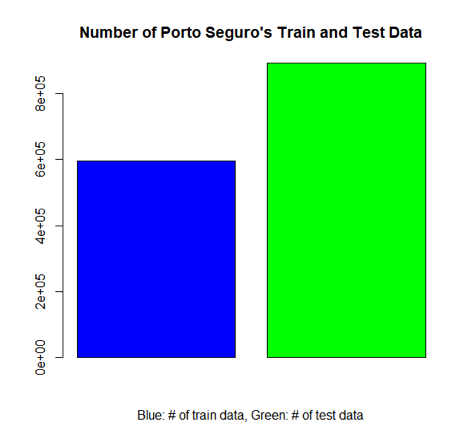
\includegraphics[width=6cm]{Intro_pic.png}
\caption{Number of objects from Porto Seguro’s given data}
\end{figure}


\bigskip
\bigskip

%----------------------------------------------------------------------------------------
% Approach and Algorithms
%----------------------------------------------------------------------------------------

\section{Approach $\&$ Algorithms} % The \section*{} command stops section numbering


\subsection{Handling Data}
\hspace{\parindent} To train a  machine with the given data, we have to handle the missing values in both data. We used the function na.omit to handle the NA values in data. But the number of objects didn’t change, thus we found out that there are no NA values in the data. \\
We figured out ‘-1’ indicates missing values in Porto Seguro’s data. By using function unique, we could get the number of missing values. Train data has 470280 missing values out of 595212 objects, which means 79.0105$\%$ of the data are missing values. And test data has 706249 missing values out of 892816 objects, which is 79.10353$\%$. Because number of missing values are excessive, we could not ignore the missing values
\begin{figure}[h]
\includegraphics[width=7cm]{approach_im1.png}
\includegraphics[width=7cm]{approach_im2.png}
\caption{Number of invalid and valid data in Train and Test data}
\end{figure}
\\ \\
\hspace{\parindent} We decided to substitute the missing values with the average value of each column. We compute the average value after we eliminate ‘-1’ values, because ‘-1’ will cause wrong average value of each column. \\
After we decided to substitute missing values to average value of each column, we need to make decision what columns do we need compute. Because if we compute all column’s average, then it will increase the run-time a lot. We decided not to compute the binary columns, because binary columns only contain 0 and 1, and didn’t have any ‘-1’ values, we didn’t compute the average values for binary columns. 
\begin{figure}[h]
\includegraphics[width=8cm]{approach_im3.png}
\caption{Train data’s correlation plot}
\end{figure}
\\ \\

Most controversial problem was computing calculated features’ average or not. Because figure 4 explains calculated features are mostly unrelated columns to target and given calculated features are not raw data, we thought we need to eliminate the calculated features. \\
However, we still want to check it is necessary or not after we see the result. So, we decided to create two different data frame variable; one for holding calculated features, and another for eliminating calculated features. 

After we got the average value of each column for two different data, we created the categorical arrays which will contain the name of the columns of each data. By using categorical array, we could insert the average value to missing values
\begin{figure}[h]
\includegraphics[width=8cm]{approach_im4.png}
\caption{Before substituted to average in train data}
\end{figure}

\begin{figure}[h]
\includegraphics[width=8cm]{approach_im4.png}
\caption{After substituted to average in train data}
\end{figure}

\subsection{XGBoost}
\hspace{\parindent} XGBoost or Extreme Gradient Boosting is a Greedy Function Approximation using a gradient boosting machine. It is an open-source tool which we used to predict the values for this Porto Seguro project. To understand the XGBoost we need to know about supervised learning and gradient boosting decision tree algorithm .
\\ Supervised learning is a type of machine learning where we have training data with multiple features x$\_$i  to predict a target variable y$\_$i. \\
The model of XGBoost is a tree. The tree ensemble model is a classification and regression trees. A model in supervised learning usually refers to the mathematical structure of how to make prediction. 
Boosting is an ensemble technique where new models are added to correct the errors made from existing prior models. This process is repeated until no improvements are made between the models.
Gradient boosting is where new models are created that predict the errors of prior models and then conglomerated together to make the final decision model. The difference between boosting is that it minimizes the loss when adding new models. 
\\ XGBoost is a tool motivated by the formal principle of gradient boosted decision tree. The goal of this library is to push the extreme of the computation limits of machines to provide a scalable, portable and accurate library.
\\ We used the XGBoost library after cleaning the data. We first created a test data as a matrix, which didn’t have the ID and target features. Before moving on to the next step, we needed to decide on the parameter and the best number of iterations. The parameter for this project was the ETA value or the learning rate, the ETA value is important because when we choose a good eta value it can prevent overfitting. The value is in the range from 0 to 1. In XGBoost it’s usually best to keep the ETA value as low as possible. And iteration had to kept large since we wanted to test the data set as much as possible


\subsection{K-Nearest Neighbors}
\hspace{\parindent} KNN is efficient classification algorithm and predict the result with binary value 0, and 1. It calculates the distances of each objects and find the nearest neighbors of each objects. After find the nearest neighbors, it creates the centroids of each neighborhoods, and classify the data. We decide to use this algorithm to see how accurate it is. 

We make our KNN code with train data, test data, and k-value as inputs. We choose calculating distance method to Euclidean.

\begin{figure}[h]
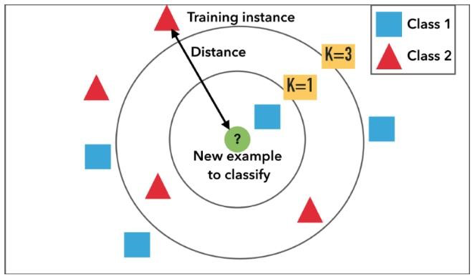
\includegraphics[width=9cm]{knn.png}
\caption{Visualization of K-Nearest Neighbors Classification. }
\end{figure}
\bigskip
\bigskip
%----------------------------------------------------------------------------------------
% Experiments
%----------------------------------------------------------------------------------------


\section{Experiments}
\hspace{\parindent} We need to test with different eta value, number of iteration for the XGBoost for both data included calculated features, and data eliminated calculated features. Then we will compare the best result from XGBoost and KNN result.


\subsection{Including calculated features result}
XGBoost with eta= 0.01, iteration=700 gives score 0.27444 \\
XGBoost with eta= 0.01, iteration=800 gives score 0.27528 \\
XGBoost with eta= 0.01, iteration=900 gives score 0.27529\\
\\ 
XGBoost with eta= 0.03, iteration=700 gives score 0.27087\\ 
XGBoost with eta= 0.03, iteration=800 gives score 0.26940\\ 
XGBoost with eta= 0.03, iteration=900 gives score 0.26789\\

\subsection{Eliminating calculated features result}
XGBoost with eta= 0.01, iteration=700 gives score 0.27488\\
\textbf{XGBoost with eta= 0.01, iteration=800 gives score 0.27650}\\
XGBoost with eta= 0.01, iteration=900 gives score 0.27632\\
\\
XGBoost with eta= 0.03, iteration=700 gives score 0.27059\\
XGBoost with eta= 0.03, iteration=800 gives score 0.27059\\
XGBoost with eta= 0.03, iteration=900 gives score 0.26919\\

\subsection{Deciding XGBoost or KNN}
\hspace{\parindent} We could get the result from KNN after 15 hours from when we run the code. It’s running time is extremely long, and this running time give enough reason why we need to choose XGBoost rather than KNN. \\
KNN doesn’t rate the target with the probabilities. It rates the target with binary value, 0, and 1. So we could get only the error rate from KNN. \textbf{We choose to run KNN with k value to 3, and the error rate was 0.002888613} which is highly accurate. However, because of extremely long running time, and format of the result, we decide to use XGBoost rather than KNN.



\bigskip
\bigskip
%----------------------------------------------------------------------------------------
 % Results
%----------------------------------------------------------------------------------------
\section{Results}
\hspace{\parindent} From Step 3. Experiment, we found out using XGBoost algorithm gives better result than K-Nearest Neighbors algorithm. The run time of KNN was much longer than XGBoost, and also gave worse result. 
And also, as we predicted on Step 2.1: handling data’s Figure 4, eliminating calculated features gives better result than including calculated features.\\
By when experimenting with different eta value and number of iteration for XGBoost, scores increase when eta decrease from 0.03 to 0.01, and gives better result when number of iteration is between 700 and 900. So number of iteration must be proper number and eta value should be small number.\\
XGBoost with eta value 0.01, iteration with 800 times, objective to “binary:logistic”, booster = “gbtree” gives best score 0.27650. \\
And by using xgb.importance function, we could rank each features’ importance except calculated feature. \\ \\ \\
Most top 10 important features are: \\
$ps\_car\_13, ps\_reg\_03, ps\_ind\_05\_cat, ps\_ind\_03, ps\_ind\_15, \\
ps\_ind\_17\_bin, ps\_reg\_02, ps\_reg\_01, ps\_car\_14, and \\
ps\_car\_01\_cat.$


\bigskip
\bigskip
%----------------------------------------------------------------------------------------
 % Conclusions
%----------------------------------------------------------------------------------------
\section{Conclusions}

\hspace{\parindent} We concluded our project with the 0.27650 score from Kaggle, which is near the top 50$\%$ percentile of the submission. While working on this project our team faced many challenges, the run time on the program was extremely long, we didn’t have a big and fast enough processor to run the code which delayed us a lot during the experimenting process. Moreover, the KNN algorithm that we worked with took more than 14 hours to compute the result which made us difficult to test out different values. Overall, we found out that XGBoost was the go to method to work with data mining, and eta value 0.01 and iteration of 800 times gave us the best score. 


\bigskip
\bigskip
%----------------------------------------------------------------------------------------
% Challenges
%----------------------------------------------------------------------------------------
\section{Challenges}

\hspace{\parindent} There were lots of hurdles we faced during this project. And all of the challenges were caused by huge data size. Train data has 595,212 rows with 59 columns, and test data has 892,816 rows with 58 columns. When we run the XGBoost algorithm to each of the data, it took more than 10 minutes. So it was hard to get all the scores from different eta value and iteration number. \\ \\
After we score all the results from XGBoost, we faced the real huge problem. It was KNN. We could get the result from KNN after 15 hours of running time

\bigskip
\bigskip
\bigskip



\phantomsection
\section*{References} % The \section*{} command stops section numbering

\addcontentsline{toc}{section}{References} % Adds this section to the table of contents



%----------------------------------------------------------------------------------------
%	REFERENCE LIST
%----------------------------------------------------------------------------------------
\phantomsection

\hspace{\parindent} 1. Bronshtein, Adi. “A Quick Introduction to K-Nearest Neighbors Algorithm.” Medium, Medium, 11 Apr. 2017, medium.com/@adi.bronshtein/a-quick-introduction-to-k-nearest-neighbors-algorithm-62214cea29c7. \\

 2. Brownlee, Jason. “A Gentle Introduction to XGBoost for Applied Machine Learning.” Machine Learning Mastery, 17 Aug. 2016, machinelearningmastery.com/gentle-introduction-xgboost-applied-machine-learning/.

\bibliographystyle{unsrt}
\bibliography{sample}

%----------------------------------------------------------------------------------------

\end{document}